\chapter{Domain Adaptation} \label{ch:domainAdaptation}
In computer vision, there are situations in which we only have access to a dataset for training but to other similar dataset for testing. Generally, collecting more data needs more resource. Sometimes, collecting data in the target condition is inefficient or even impossible so training models on existing data is preferable. In these situations, simply training on the given images without further adjustment can result in bad performance, for example inaccurate prediction in object classification task. This is because even if the images represent similar objects, they are still different in e.g. the quality of the images, the backgrounds or if they are still images or from video \cite{shiftImgVid}. 

\subsection*{Definitions of Domain Adaptation}
Generally, the domain from which we have supervised data is called the 'Source Domain', subscripted with $s$, and the domain in which we want the machine to perform classification the 'Target Domain', subscripted with $t$. Given a training set with samples $\left\{x_s^i, y_s^i\right\}_{i=1, ..., n_s}$ and a test set with  $\left\{x_t^i, y_s^t\right\}_{i=1, ..., n_s}$ from the source and target distribution $\mathcal{D}_s$ and $\mathcal{D}_t$ accordingly, applied from \cite{DAnetwork}, the goal of domain adaptation is to predict the classification $\hat{y}_i$ when $\mathcal{D}_s \neq \mathcal{D}_t$ and with little to no supervised samples from the target domain. If there is supervised samples from the target domains, it is the case of supervised domain adaptation. In semi-supervised domain adaptation, both labeled and unlabeled samples from the target domain are used in the training. Finally, if only the unlabeled samples from the target domain are present, it is unsupervised domain adaptation. In our experiment, the neural network is trained on labeled samples from the source domain and the samples from the target domains are involved without labels so the method we use is also in the field of unsupervised domain adaptation. Additionally, if the source and target domains are directly related and the domain knowledge can be transferred in only one step, this will be called one-step domain adaptation. However, if the domains are insufficiently related, there must be at least another domain acting as a bridge between the source and the target domains. This case is called multi-step domain adaptation. The existing domains in one-step, multi-step DA and traditional machine learning are visualized in figure \ref{fig:DAsteps}

\begin{figure}[tbh]
  \centering
    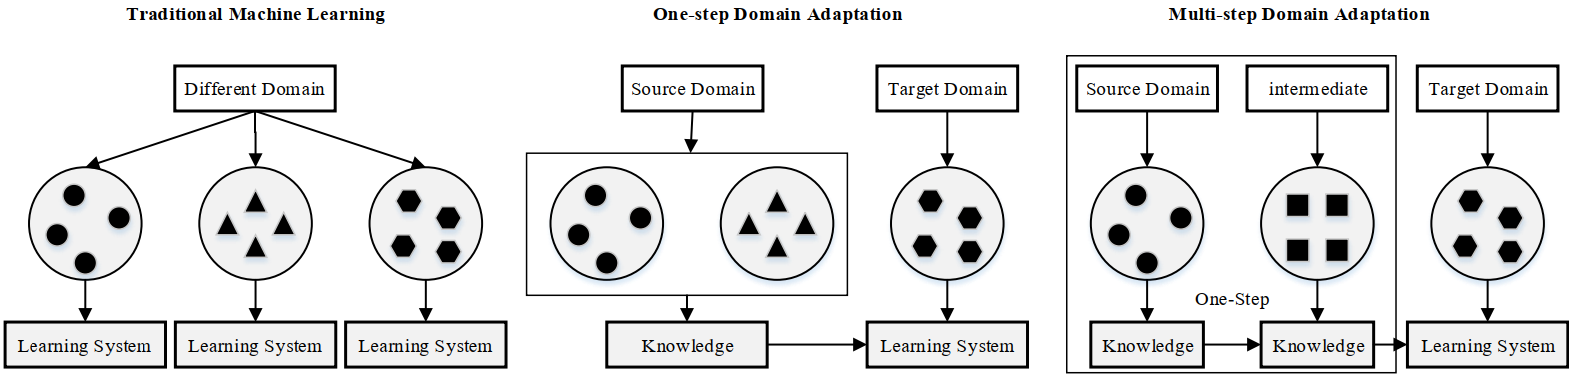
\includegraphics[width=\textwidth]{abbildungen/DAsteps.png}
  \caption{Knowledge transferring in types of Domain Adaptation \cite{deepDASurvey}: Different domains are involved differently in traditional machine learning (a), one-step DA (b) and multi-step DA. In traditional machine learning, each domains are used to train separately. In one-step DA the knowledge from source domains can be transferred directly to the target domain, whereas the multi-step uses another domain more similar to the target domain as an intermediate domain in the transfer.} 
  \label{fig:DAsteps}
\end{figure}

These differences between the domains present itself to a system as different distributions among the datasets - by changing the dataset, we also change the distribution of the data the system uses. This change of the distribution is called dataset shift and the datasets with different distributions are referred to as being from different domains. It is useful to understand how this happens before proceeding with solving this problem. In the next section, the cause of the different domains, the dataset shifts, will be discussed. 

\section{Dataset Shifts} \label{sec:datasetShifts}
In collecting data, there are many aspects that can in influence the characters of the data. To name examples related to image data, the lighting condition, for instance, can generally change the overall intensity of the pictures: the pictures take in a dark room will generally have lower intensity value than in the ones taken in sunlight regardless of which objects are captured. This shows an example of how the environment can change the underlying distribution of the input value. Another possible cause of a dataset shift is how the samples are selected to be in a dataset. It is understandable that a data collection is built up of the inputs of similar nature. This is referred to as the sample selection bias.

The insimilarities between the distributions, the dataset shifts, are categorized after the source of the shifts. In \cite{shiftinML} and \cite{shiftDataset}, the shift types are defined differently: in \cite{shiftinML} they are splitted after common causes of the shifts whereas in \cite{shiftDataset} they are splitted more generally after the change in probability distribution the shifts cause. Now, we will discuss different types of the dataset shifts according to \cite{shiftDataset}. To understand this, it must be mentioned first that the joint distribution $p(x, y)$, the probability that both x and y occur, can be calculated by:
	\begin{equation}\label{eq:jointXY}
			p(x, y) = p(x | y)p(y) = p(x | y)P(x)
	\end{equation}

According to this equation, the possible dataset shifts occur when $p(x)$, $p(y)$ or $p(x|y)$ changes which results in covariate shifts, prior shifts or concept shift respectively. 

\subsubsection*{Covariate Shifts}
The covariate shifts are caused by different distributions of the input between the domains whereas the conditional distributions of the output given the input are the same. This kind of shift is possible in a $X \to Y$ problem where y is dependent on x and occurs when $p(x)$ changes and the conditional probability $p(y|x)$ stays the same. This shift is a very commonly studied in the problem of domain adaptation. The covariate shifts include the case when the sampling is biased as mentioned above as the sample selection bias. This is the same as when the political survey is done to create a prognosis about the upcoming election, in an area where one political party invests more on running a campaign, the result would be more in favor of that party than in another area. The result of this area is not necessarily the real opinion of the majority of the people in that country. 
Another possible cause of the covariate shifts is when the data is missing from the collection which alters the probabilities of the remaining samples in the dataset. Having less representations of something could rise the probability of another thing in the same sample. The effect of the change is visualized in figure \ref{fig:covariateShiftPic}
\begin{figure}[tbh]
  \centering
    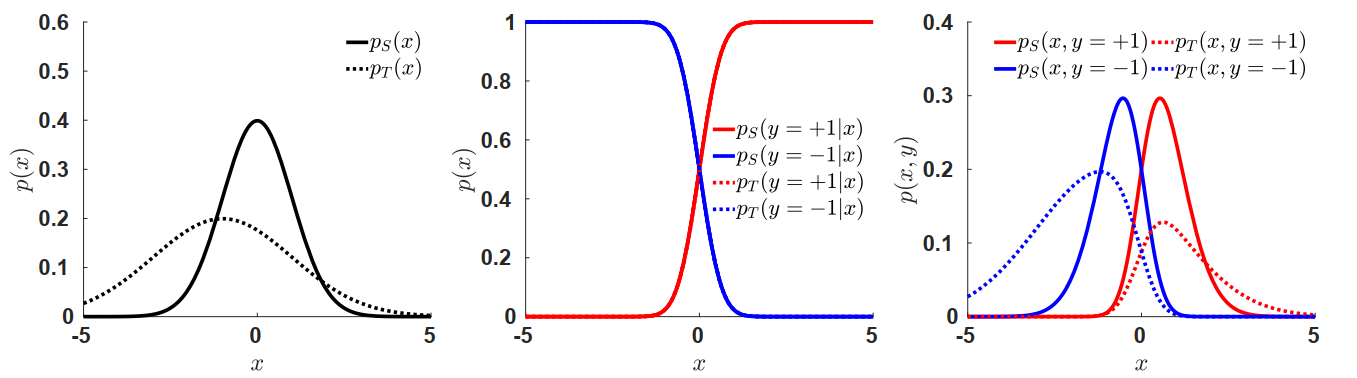
\includegraphics[width=\linewidth]{abbildungen/covariateShiftPic.png}
  \caption{Covariate Shift \cite{dataShifts}: There is a shift in the data distribution (Left) from the target (in the picture $p_T$) to the source (in the picture $p_S$) whereas the posterior distributions (Middle) are similar. As a result, the joint distributions (Right) are shifted.}
  \label{fig:covariateShiftPic}
\end{figure}

\subsubsection*{Prior Shifts}
The prior shifts, on the other hand, occur when the districution of the output changes, i.e., when $p(y)$ changes whereas the conditional probability $p(y|x)$ stays the same. This would also cause the joint distribution $p(x, y)$ to change. Practically, this shifts happen when the rule of the classification changes, for example, the level of toxic detected before it is classified as dangerous. If we take the sample from the same water, the composition of the water might not change but by changing the detection rule, the probability of the same water being toxic might alter if the threshold is changed. The visualization of the change in this distribution is to be seen in figure \ref{fig:priorShiftPic}.
\begin{figure}[tbh]
  \centering
    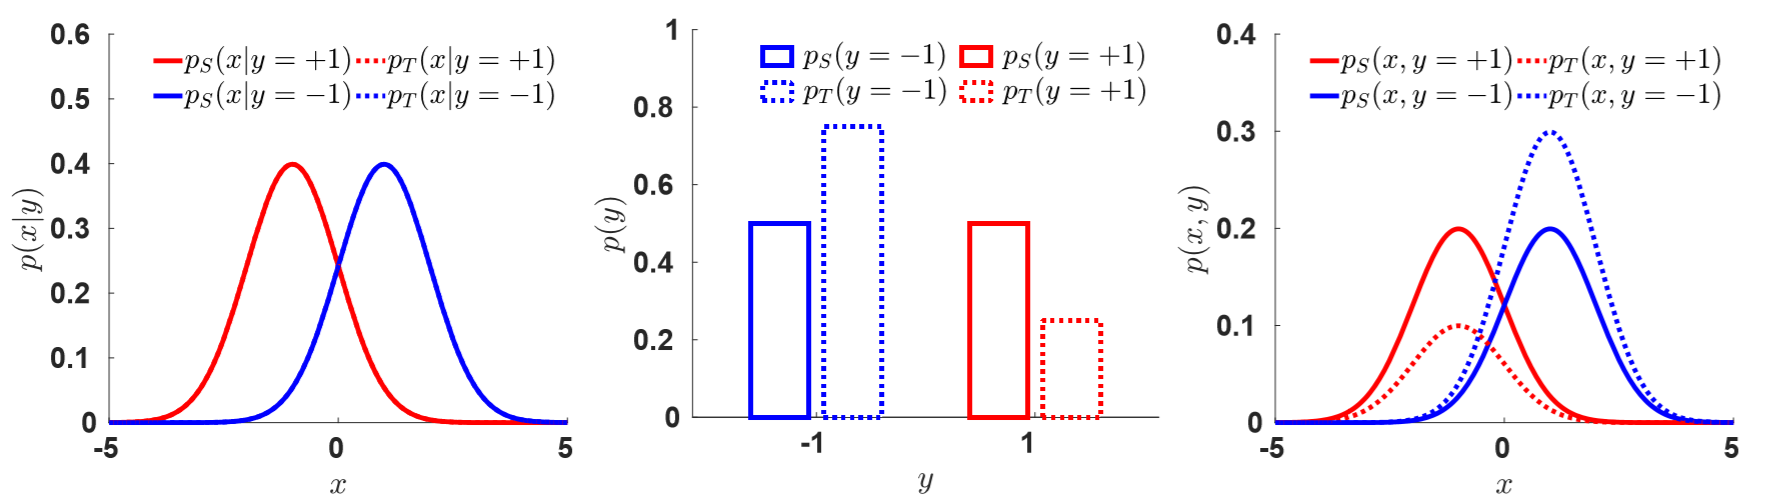
\includegraphics[width=\linewidth]{abbildungen/priorShiftPic.png}
  \caption{Prior Shift \cite{dataShifts}: The distributions of the positive and negative class label are similar within the training and testing set (Left) but due to the differences in probabilities $p_s \neq p_T$ (Middle), the joint probabilities are not equal in the testing set (Right)}
  \label{fig:priorShiftPic}
\end{figure}

\subsubsection*{Concept Shifts}
The concept shifts are different than two previous shifts. Here, the data distributions $p(x)$ and $p(y)$ are the same while the conditional distribution $p(x|y)$ changes. These shifts are common in reality since the nature of the conditions always changes. For example, forecasting weathers in different seasons also have different criterion. Figure \ref{fig:conceptShiftPic} illustrates this change and its effect on the joint distribution. 
\begin{figure}[tbh]
  \centering
    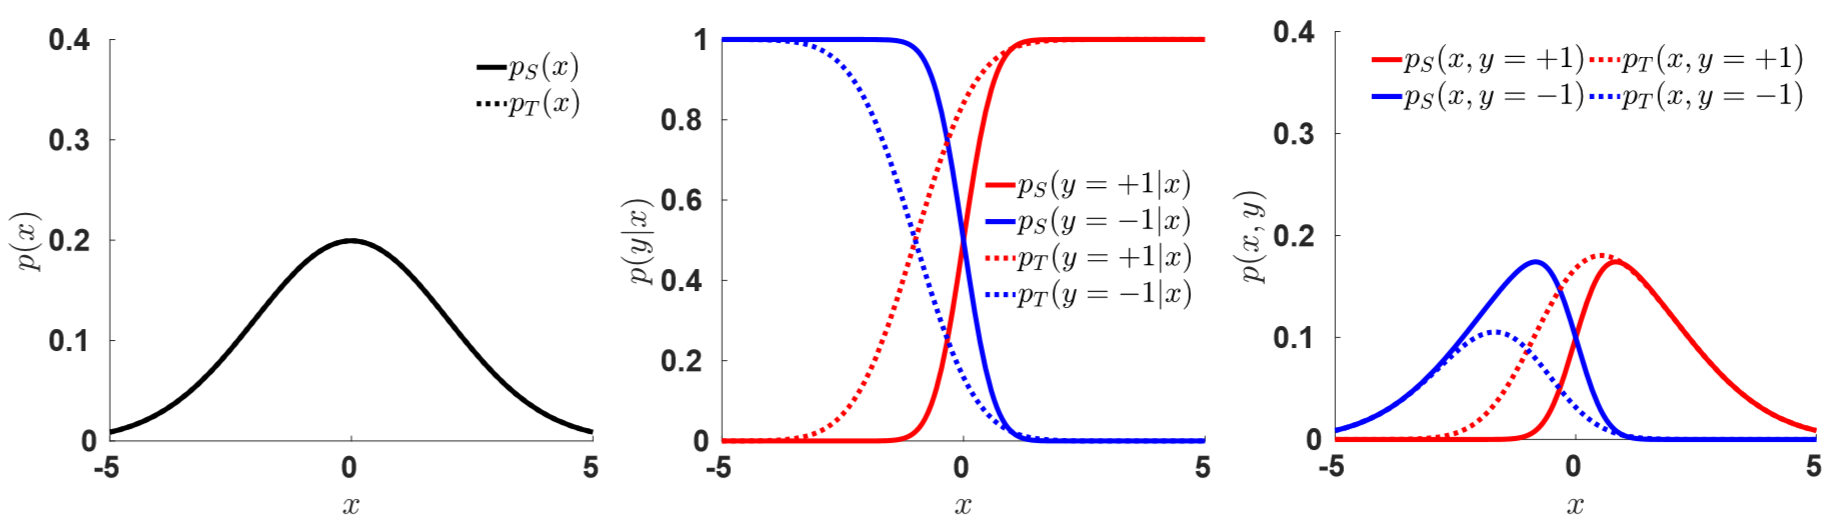
\includegraphics[width=\linewidth]{abbildungen/conceptShiftPic.png}
  \caption{Concept Shift \cite{dataShifts}: The data distributions in the source and the target set are the same (Left) but the shifts in $P_T(\vec{Y}|\vec{X})$ from that of the source target (Middle) cause a shift in the joint distribution (Right).} 
  \label{fig:conceptShiftPic}
\end{figure}

Due to these introduced shifts, datasets can have different data distribution. Since traditional classifier is not adaptive when it is trained on data from one domain and the testing is done on another domain, Domain Aadaptation (DA) is introduced to solve this problem. 

Mostly, the studied cases of domain adaptation assume complete source and target domains. However, there exist situations in which the involving domains are combinations of different domain. These scenarios are referred to as the Domain Mixture Scenario \cite{domainMixture}. In the next section, this particular scenario and its variations will be explained.


%Domain Mixture Scenario
\section{Domain Mixture Scenario} \label{sec:domainMixture}
Domain adaptation improves the performance of a network when the training is done on a dataset and the tasks should be performed on another dataset with different data distribution. This enables using similar data as the training data when the target data is entirely not available or just sparsely available. Ideally, the domain from which we have plenty of data should already contain a complete set of data i.e. samples of all classes we want to classify. If this is the case, the model will have a uniform data distribution to learn both the object representations and the domain information effectively. For example, creating 3D models can offer training images for all objects more efficiently than to actually capture the images of those objects from the real world. To be able to use these synthesized images as training data despite the real performance being planned for the real-world images, domain adaptation can be used to account for the different character of these images. Furthermore, it is also possible to have multiples classes serving as the training set. There might be, for instance, existing image collections of the same objects taken under different conditions that can be combined together to build up bigger training dataset than by using only one collection. 

In reality, a dataset might contain data from several different domains. For example, we might have images captured with different cameras or in different locations. It is also possible that each domain only contains parts of the possible classes and needs to be used together to create a dataset with complete class representations. This case of domain adaptation with multiple sources pose another challenges since there are now many data distributions in one source domain that should be approached differently from the situations with only a single domain acting as a source domain. To have an overview of this special situation, we will now briefly describe previous studies on these scenarios with many source domains.

\section*{Previous Experiments on Multi-source Domain Adaptation}
Most researches done on domain adaptation look into cases in which the domain transfer bridges one source domain to the target domain. However, if there are data from several domains available, using them all would give the model more useful data to work on than using just one domain. One possible way to use them is to combine them into one single source domain. By doing this, their differences might not be accounted for effectively enough \cite{multisourceDAsurvey}. Another possible way is to train several models solely on each one of the available domains, then to combine them into a model that can perform well on the new domain. \cite{multiDAclassi} developed the Domain Adaptation Machine (DAM) which learns to classify data in the target domain using classifiers pre-trained separately on the labeled samples from the source domains called auxiliary or source classifiers. The target classifier is optimized to make accurate predictions by adjusting weights applied on these auxiliary classifiers of each source domain. Its optimization aims to reduce the difference between the decision value of the target classifier and the source classifiers on the labeled source data. At the same time, the DAM also trains to minimize the decision error of the target classifier on the labeled target data if available. Figure \ref{fig:auxclassifiers} shows the structure of multi-source domain adaptation with separate source classifiers.

\begin{figure}[tbh]
  \centering
    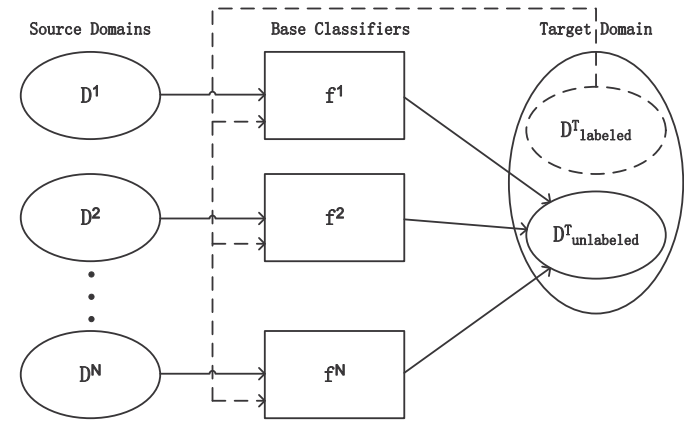
\includegraphics[width=0.8\textwidth]{abbildungen/multiDAclassi.png}
  \caption{Multi-source Domain Adaptation: Each classifier is trained on each available domain and labeled target data if possible. Then, they are combined to make accurate prediction on the unlabeled data in the target domain. \cite{multisourceDAsurvey}}
  \label{fig:auxclassifiers}
\end{figure}

The two mentioned methods require the domain labels of the data. In some situation in which we have a mixture of several unknown domains, for example, pictures from an internet search with many unknown origins. To support using these samples, \cite{multiDAcluster} proposed finding clusters representing domains in the data to acquire their domain labels. They also adapt a domain transformation method to the problem with multiple source domains. This original cross-domain transformaton \cite{multiDAcrosstrans} learns to find a transformation from a data point in a domain to the other and even works when not all the class samples in the target domain are in the training set - a very common situation when dealing with real-world data. 
 
In practice, the data serving as domain happens to lack elements of some classes and we may need to combine data from multiple domains to get a complete set of class representations as shown in figure \ref{fig:imsDA}. \cite{multisourceDA} published in 2018 also addressed insufficient exploration of the incomplete multisource transfer learning (IMTL) where none of the sources domain is complete. They proposed using low-rank transfer subspace to assist learning features from multiple domains. A subspace is a model suitable for describing the underlying characteristics of a dataset and a good way of realistically describing the nature a dataset is by using multiple subspaces \cite{subspaces}. Finding a shared subspace between source and target domains is one method of applying domain adaptation. With multiple sources, their different distributions must also be taken into account. Further from finding a domain-free subspace by finding low-dimensional features representing different classes, they reconstruct the missing class data of each source domain through this shared subspace with the information from the complete target domain - they learn from each other in both ways. 

Partly, the experiments in \cite{multiDAcrosstrans} and \cite{multisourceDA} assume, similarly to the domain mixture scenario, incomplete domains involving in the training phase - the datasets shown during the training have labeled samples of only subsets of all the competing classes. A difference is that \cite{multiDAcrosstrans} also include some labeled samples of the target which are not labeled at all in the domain mixture scenario. However, \cite{multisourceDA} also includes only unlabeled target samples. A crucial variation in our experiments, similar to \cite{domainMixture}, is the investigation on the varying ratio of the labeled samples to the unlabeled samples from different domains in the mixture. 

\begin{figure}[tbh]
  \centering
    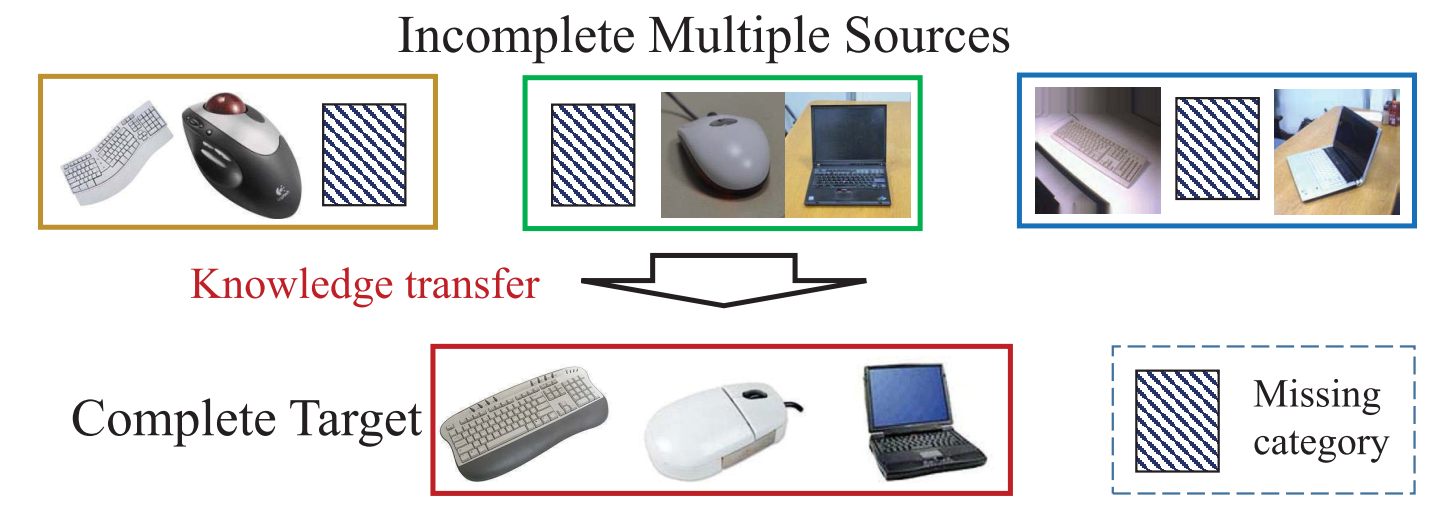
\includegraphics[width=\textwidth]{abbildungen/IMS-DA.png}
  \caption{Domain Adaptation with Incomplete Multiple Sources: Sometimes, we must combine multiple domains to have complete samples of all possible classes existing in the target domain. \cite{multisourceDA}} 
  \label{fig:imsDA}
\end{figure}

In this thesis, we investigate the scenario of domain adaptation as present in \cite{domainMixture} where there are supervised samples of all competing classes but they are not all from the same domain. This scenario actually represents the reality. A complete image collection of objects taken under the same condition, with the same camera model or pictures drawn or generated in the same style are created mostly for researches. In reality, we might find pictures of some objects taken under one condition and others taken under another. \cite{domainMixture} is also motivated by several operating house robots which serve in different areas in the house. A robot responsible for the kitchen might have captured a picture of a knife and a mixer while a robot serving in the bedroom might have pictures of a pillow the first one has never captured. On the other hand, the dog roaming around the house probably has been captured by both. It’s also realistic to imagine that both rooms have different light setting and the robots have different models of camera, then the pictures of each object will also come from different domains. Then, it is also possible that the images of some objects under a capturing condition are already labeled and others are not. Possibly and ideally, all the objects might appear in all the domains involved. As we can see, there are many possibilities of how the situation of the image collection usable as a training dataset can be.   

Of interest are the cases in which there is a complete set of supervised samples representing every possible classes we can use as a training set. However, these supervised samples are not all from the same domain and none of the domain has supervised samples of all the classes - the samples from both domains must be mixed in order to create a full representation of the classes. In \cite{domainMixture}, two versions of this scenario are investigated:  
\subparagraph*{Complete Domain Mixture: } Here, apart from the supervised data from some classes, the domains also have unsupervised samples of the remaining classes. In other words, all the domains have a complete set of samples with all the classes but they are only partly supervised.      
\subparagraph*{Sparse Domain Mixture: } In this variation, combining the supervised samples from all the domains still yield a set with all the classes but each domain has unsupervised samples of only parts of the missing classes. 
These two different scenarios of domain mixture are shown in Figure \ref{fig:scenarioDA}. 

\begin{figure}[tbh]
  \centering
    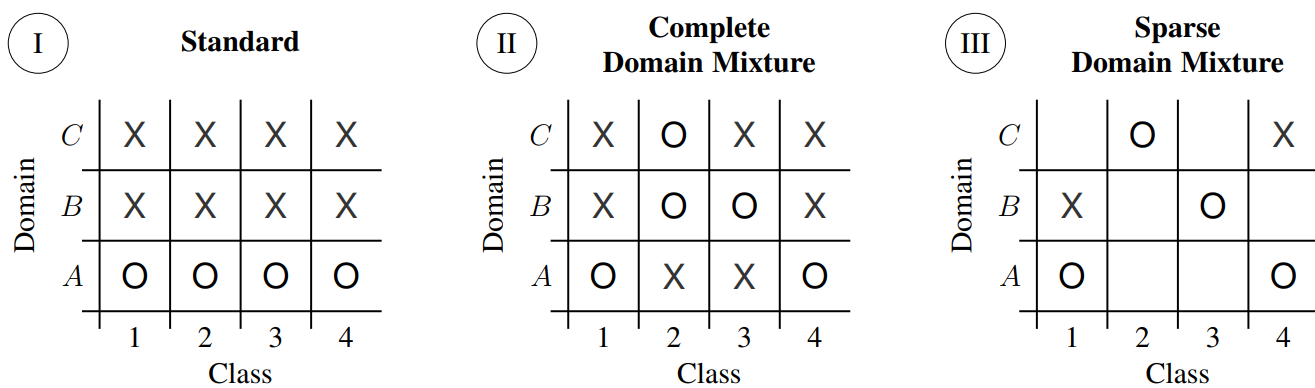
\includegraphics[width=\textwidth]{abbildungen/scenarioDA.png}
  \caption{Different Domain Mixture Scenarios \cite{domainMixture}: Present classes in the domains (A, B, C) are different in each scenario. The classic case of domain adaptation (left) is when we have a complete set of supervised data from one domain and want to learn to transfer the knowledge to other unsupervised domains which are also completed. The domain mixture scenarios also have supervised samples from all competing classes but only the complete one (middle) also has unsupervised samples from the missing domain-class combinations whereas the sparse one (right) lacks some combinations entirely.}
  \label{fig:scenarioDA}
\end{figure}

These scenarios are challenging since the objects are known to the network only in one variation from a domain, and some objects in other variation. The network has less information on what is domain-specific or what is object-specific. Intuitively, if we take different backgrounds as different domains and we want to tell what object is in the pictures, we would have to know what identifies the object and what comes from the background. We would make an assumption to what the object is, then we would look for the same object with different background to be able to confirm our assumption. In the domain mixture scenario, the model might only have seen an object and been told by the label what object it sees, then it would try to learn which features signalize the object. However, since it only has labeled pictures of that object with one background, it cannot directly compare what features are common when the backgrounds are different. Instead, it must try to extract background-specific features from the mixed data available and then learn aspects of the image that is independent from the backgrounds which should be relevant to the object itself. This is also already proposed in a theory on domain adaptation that the domain-irrelevant representations enable the best condition for a domain transfer the classifier needs  \cite{DArepres}.

With the knowledge about the domain adaptation and especially the domain mixture scenario, the next section will describe the DSN, how it applies domain adaptation with its components and why it might be a good choice to tackle these scenarios.